
\documentclass[12pt]{article}


%%% PACKAGES

\usepackage[pdftex]{graphicx}

\usepackage{hyperref}
\usepackage{bibentry} %to use intext full bibliography entries instead of citations.  You will need a separate BibTex database for this to work.  See http://cst.usc.edu/services/tel/grants/legrants.html for details on this package.
\usepackage{booktabs} % for much better looking tables
\usepackage{array} % for better arrays (eg matrices) in maths
\usepackage{paralist} % very flexible & customisable lists (eg. enumerate/itemize, etc.)
%\usepackage{verbatim} % adds environment for commenting out blocks of text & for better verbatim
%\usepackage{subfigure} % make it possible to include more than one captioned figure/table in a single float

\usepackage{caption}

\usepackage{color}

%%% PAGE DIMENSIONS
\usepackage{geometry} % to change the page dimensions. Read ftp://ftp.tex.ac.uk/tex-archive/macros/latex/contrib/geometry/geometry.pdf for detailed page layout information 
\geometry{margin=1in} % for example, change the margins to 1 inches all round
%\geometry{landscape} % set up the page for landscape
% 

%%% HEADERS & FOOTERS
\usepackage{fancyhdr} % This should be set AFTER setting up the page geometry
\pagestyle{fancy} % options: empty , plain , fancy
\renewcommand{\headrulewidth}{0.4pt} % customise the layout...
%\lhead{}\chead{}\rhead{}
%\lfoot{}\cfoot{\thepage}\rfoot{}

%\rfoot{\footnotesize SIR 330}
\rhead{\footnotesize BME 3300 Project Guide}
\renewcommand\footrulewidth{0pt}

\usepackage{enumitem}
%%% SECTION TITLE APPEARANCE
%\usepackage{sectsty}
%\allsectionsfont{\sffamily\mdseries\upshape} % (See the fntguide.pdf for font help)
% (This matches ConTeXt defaults)


%% END Article customise

%%% BEGIN DOCUMENT


\begin{document}


\thispagestyle{plain} %alternatively specify empty to get no footer on first page.  This is part of the fancyhdr package


\nobibliography{MasterBib} %this specifies the BibTex directory that stores your desired bibliography entries.  It has to come before any \bibentry lines are invoked

\bibliographystyle{apalike} %be careful here, there is only a few styles that will run


%\tableofcontents
\begin{center}

\textbf{BME 3300 Project Guide} \medskip

\end{center}

\section*{Objective} Now that you have gained some experience in the first labs building various amplifier and filter circuits and making measurements,
it is time to apply those skills to build, evaluate and optimize a biomedical instrument. 
What follows is a list of potential projects, but it is not exhaustive - if you have an idea for something you'd like to build, 
talk to the TA and I about it and we can likely come up with a plan for it. 
Consult the grading rubric for the components that make a ``good'' project. 
%Basically, any project you do should comprise a characterization of the signal from your transducer,
%a circuit design that makes that signal fit the ADC of the NI breakout board or Arduino and (if necessary) suppresses noise,
%and some processing in LabView or on the microcontroller to derive and display useful results.

\section*{Schedule}
\begin{itemize}
\item Week of October 19th: Choose a project, discuss with professor and TA, and develop parts list. Start working!
\item Weeks of October 19th-November 30th: Work on projects.
\item December 7: Project Presentations.
\end{itemize}

\noindent From time to time we will schedule additional lab time (outside of the normal Monday time) to work on projects,
subject to demand, availability of the room, and availability of the TA or professor.

\section*{Concepts worth considering}
\begin{enumerate}
\item CMOS chip run on 5-12V and ground. TTL chips run on 5 volts max. Check this first!
\item The op amps we have in lab require symmetric power. You cannot run them off +5 volts and
ground.
\item Decoupling capacitors for each op amp and IC should be included in any circuit combining
digital and analog components.
\item There is rarely a reason for AC coupling your scope. Doing so often hides the real problem.
\item Build your device MODULARLY and check sections as you go. 
Check functionality after adding each component. 
Do not wire the whole thing up and expect it to work.
We cannot stress this point enough, and it holds for both circuits and code. 
\end{enumerate}

\newpage 

\section*{Project 1: MRI RF Coil}

There is a 0.5 Tesla MR magnet at one of the stations in the 3300 lab, 
along with amplifiers for transmit and received signals, and a USRP1 
software-defined radio from Ettus Instruments that is used to generate transmit signals and receive,
and digitize the incoming signals. 
Please see the 255 MR Lab info for more information about this device and how it can be used. 
The goal of this project is to build a small solenoid coil that you can drop a test tube into 
and measure MR signals. 
In doing this you will learn to use a network analyzer to tune and match the coil, 
become a pro at soldering chip capacitors,
and use the radio to acquire NMR data using your coil and a water sample. 
You will optimize the coil size and wire gauge to maximize SNR. 

\newpage

%\section*{Project 1: Digital Thermometer}
%
%In this project you will build a thermometer using a thermistor. 
%For human temperature you only need a range from 96$^{\circ}$ to 106$^{\circ}$ F.
%\begin{enumerate}
%\item You will be working with a thermistor is a wet environment. 
%You should attach insulated wires to it and then epoxy the whole connection. 
%After the epoxy sets use hot tap water, a thermometer and a multimeter to characterize R as a function of temperature over your range.
%\item Construct the bridge circuit show below with the thermistor. Set the R1/R2 such that Vout = 0 at 96$^{\circ}$.
%\item Get the thermometer working in LabView first, then implement it with a digital display using the Arduino. 
%\item Think about (and maybe implement) other ways to do the measurement, i.e., other temperature-dependent devices or circuits.
%\end{enumerate}
%
%\begin{center}
%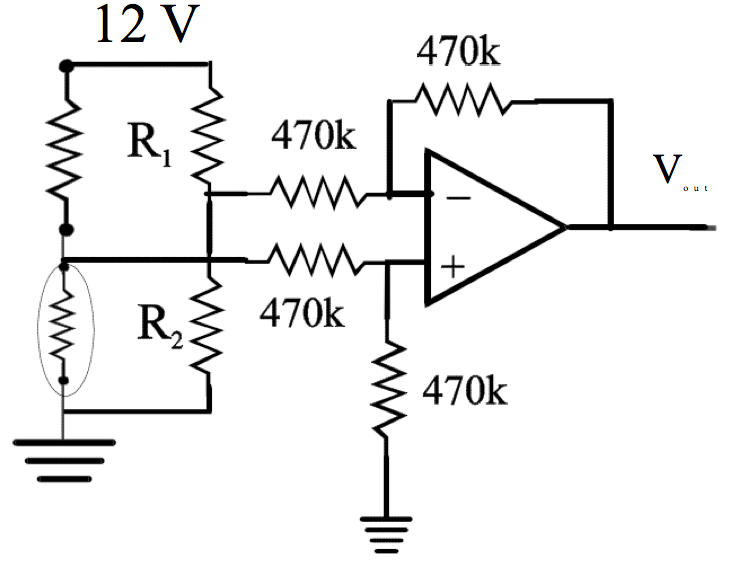
\includegraphics[width=0.75\textwidth]{thermistorbridge.png}
%\end{center}
%
%Your presentation for this project should also look at the linearity of your measurements. 
%
%\newpage

\section*{Project 2: EOG}

In this project you will build a device to measure gaze direction. 
\begin{enumerate}
\item Build two instrumentation amps such as those used in the ECG lab. You will need to tune your filters a bit.
Provide enough amplification so that looking one way and then the other causes $\approx$ 2 V swing in the output voltage. 
\begin{center}
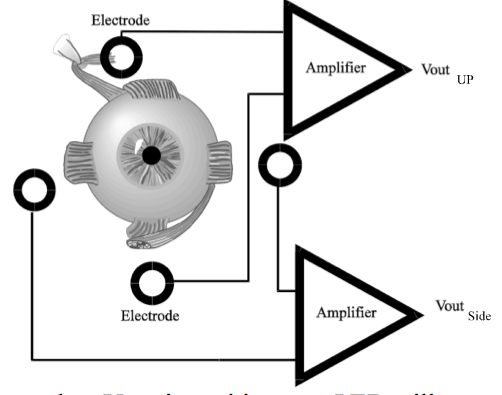
\includegraphics[width=0.45\textwidth]{EOGcircuit.png}
\end{center}
\item Plot gaze direction in real time in LabView, then build the following circuit to give a binary left-right/up-down measurement.
When $V_{out}$ is positive, one LED will light; when negative the other LED will light.
\begin{center}
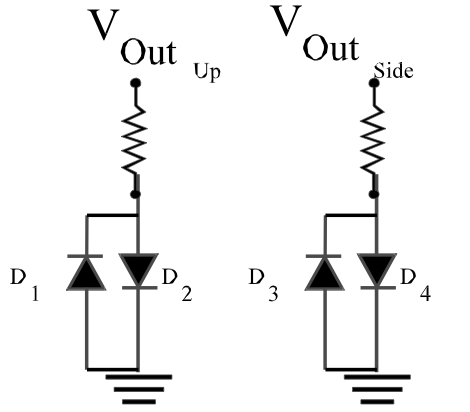
\includegraphics[width=0.45\textwidth]{EOGLEDs.png}
\end{center}
\item What else can you do with this? Could you control something (like a mouse cursor) on the computer with it? Try out a cool application.
\end{enumerate}

We have found in the past that these measurements often need to be calibrated to each subject, so be aware of that. 

\newpage 

\section*{Project 3: Pulse Oximetry}

People doing exercise want to know their heartrate and blood oxygen saturation levels.
Your task is to provide the sensors for that measurement. 
Since you don't care about ECG (you just want heart rate) you decide to use an earclip or fingerclip plethysmograph. 
Plethysmography is the measurement of volume and when your heart beats your extremities get a bit thicker (which increases their optical density). 
By shining a light through that extremity, changes in thickness are revealed as changes in emergent light. 
In addition to the heart rate, the oxygen saturation level of the blood can be measured optically. 
The oxygen saturation of blood in a healthy person is between 95-99\%. 
When it falls below 90\%, a person may pass out and if it goes low for an extended period brain damage can occur. 
Hemoglobin absorbs light differently when it is bound to oxygen. 
The absorbance differences at 660 nm and 910 nm can be measured using LEDs and a photodiode. 
A trick to avoid non-specific absorbance and eliminate the need to calibrate every time the device is moved, 
is to only measure the changes in absorbance due to the pulse. 
Hence the name ``Pulseox.''
\begin{centering}
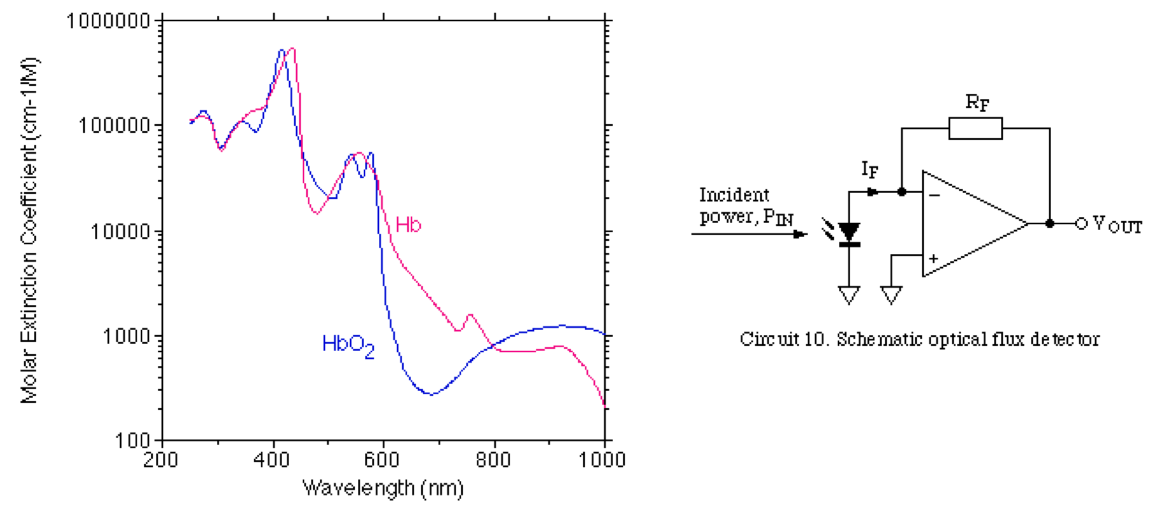
\includegraphics[width=\textwidth]{plethysmograph.png}
\end{centering}
\begin{enumerate}
\item Build and test your photodiode and light source. 
\item Apply your circuit to a vict... er subject. Set it up so that you get an output pulse per heartbeat (possibly first) in LabView but then from your Arduino. For the Arduino, make it battery powered and make or 3D print a finger clip that holds the diodes. 
\item Compute oxygen saturation by comparing transmitted light at 660 and 910 nm. 
\item Characterize the SNR of your measurements.
\end{enumerate}

\newpage

\section*{Project 4: Muscle Force Sensor}

A number of diseases, age and inaction can lead to muscle degradation. 
Measurement of strength loss or gain can be used to track either disease or recovery. 
However seeing whether someone can pick up various heavy objects, 
or how long they can hold an object lacks a little quantitative precision. 
You'd like to have something that measures both force and force over time.

\begin{enumerate}
\item Devise a system with a variable load such as a grip spring like the ones below:\\
\begin{center}
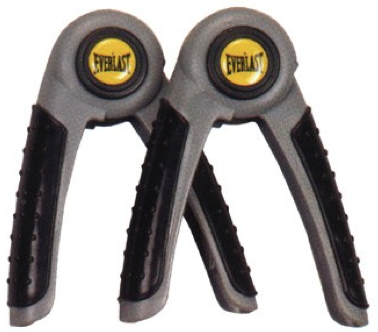
\includegraphics[width=0.4\textwidth]{gripspring.png}
\end{center}
\item Now devise a way to sense the amount of compression. 
One method would be to sense the angle between arms.
Calibrate your measurements to convert to force
\item You also want to sense the length of time of compression since someone who can flatten the arms together won't be able to hold that forever. 
Another reason for time, someone who may not be able to close it all the way but can now hold it for longer is getting stronger.
Optionally start by using LabView to measure hold time, then program an Arduino to do it with a display screen so you can make it battery powered and portable. You can also plot grip strength versus time easily.
\item Demonstrate the system with multiple users.
\end{enumerate}

This project is often chosen by students because of the simplicity of the circuit that can be developed,
however they are then foiled by the fact that it is actually rather challenging to build a robust mechanical
device to hold the sensor. 
This year we will be expecting to see a novel solution to the mechanical aspect of  this problem. 

\newpage

\section*{Project 5: Forceplate}

Force plates are used in all sorts of gait and exercise measurement. 
One way of measuring force is to apply that force to an extensible surface and measure the extension. 
Since $\Delta$length/length is strain we can measure extension using a strain gage.

\begin{enumerate}
\item Get a plate and some strain gauges, and mount the gauges on the back side of the plate 
at multiple positions.
\item Construct a bridge circuit for each of the gauges. 
Choose $R_1$ and $R_2$ such that $V_{out}$ is near 0 when the plate is unloaded:
\begin{center}
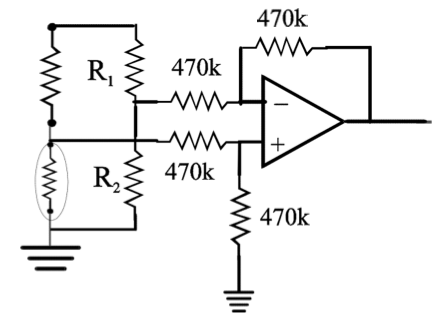
\includegraphics[width=0.6\textwidth]{forceplatebridge.png}
\end{center}
\item Add known weights to the plate, measure $V_{out}$ for each of the four plates and create a calibration load versus $V_{out}$.
You may want to add additional amplification if you aren't using the full dynamic range of your NI or Arduino inputs.
\item How linear is your device? Characterize its sensitivity.
\item Using a basketball, test the dynamic response of the plate.
\item A LabView interface will allow a sophisticated calibration and display of the measurements versus time; an Arduino interface with an LCD screen shield
will allow a bathroom scale-like display.
\end{enumerate}

\newpage

\section*{Project 6: Breathing rate sensor}

While chest expansion isn't the best way of measuring breathing rate, it is okay for home use and for triggering MR scanners. 
One technique used in the past was taking an elastic tube full of mercury and stretching it around the chest. 
As the chest expands the tube lengthens (which causes the diameter to shrink). 
By measuring the resistance of the mercury and since R= Ul/A the resistance changes as the tube length changes. 
The process of measuring changes in length by measuring changes in resistance uses devices called strain gages. 
The problem here is that mercury is expensive, heavy and toxic. 
Saline or even water can be used instead. 
Or there are things called bend sensors available, which change resistance as they are bent.

\par In every one of the methods described above, you get a resistive change which indicates your signal.

\begin{center}
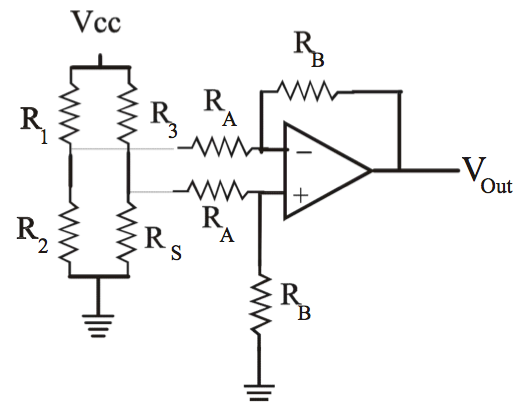
\includegraphics[width=0.6\textwidth]{breathingsensorcircuit.png}
\end{center}

Once you have an output voltage associated with the breathing signal, how do you display? 
LabView will allow you to take in pulses, 
calculate and display the breathing rate in breaths per minute, or you can count the period between breaths and display that.
If you implement this with an Arduino, you would have a great (and cheap) way to trigger an MR image acquisition. 
If you get this device working well with MR-compatible components, we could take it to a VUIIS human scanner and check whether the high magnetic field affects its operation, and monitor its output during an acquisition to reconstruct a free-breathing abdominal image free of motion artifacts.

\newpage

\section*{Project 7: Optical CT scanner}

One of the limitations of X-ray images are that they are a two dimensional representation of a three dimensional object. 
This limits the amount of information that can be discerned. 
From X-ray images we may be able to say what kind of objects we see but not their relative locations. 
But, if we rotate the X-ray relative to the objects their positions will change in each image, and we can reconstruct their
location within the body from those images. 
This is the basic idea behind Computed Tomography where multiple X-rays scans from different angles are put together to form an image. 

\begin{enumerate}
\item In the lab we have a turntable with an arm you can mount an infrared LED and detector to. 
\item Attach a potentiometer to the end of the arm to detect its position. 
\item Get both of these signals into LabView and record them as you move the arm around the object, and 
for multiple positions of the object.
\item Reconstruct a binary image using back projection. There are helpful functions in MATLAB for this.
\end{enumerate}
\subsubsection*{A little more info on Back Projection:}
Back projection is one of the most common methods for reconstructing an image. 
In a CT scanner, an X-ray source rotates around an object producing area projection data at each angle. 
That data is spread back onto an image of the area, which is divided into pixels. 
Pixels are the individual units of the reconstruction. 
Each pixel has a certain value attached to it which corresponds to the attenuation at that point. 
When put together, all the pixels reveal an image. 
As more and more X-ray scans are taken and data is back projected, an image of the area starts to emerge.
The near IR-light used in a has a larger wavelength (880nm) and lower energy. 
Infrared light is quickly attenuated by water inside the human body and is not suitable for medical imaging. 
However, it is able to pass through material with low attenuation coefficients like the light filter used in this experiment. 

\begin{center}
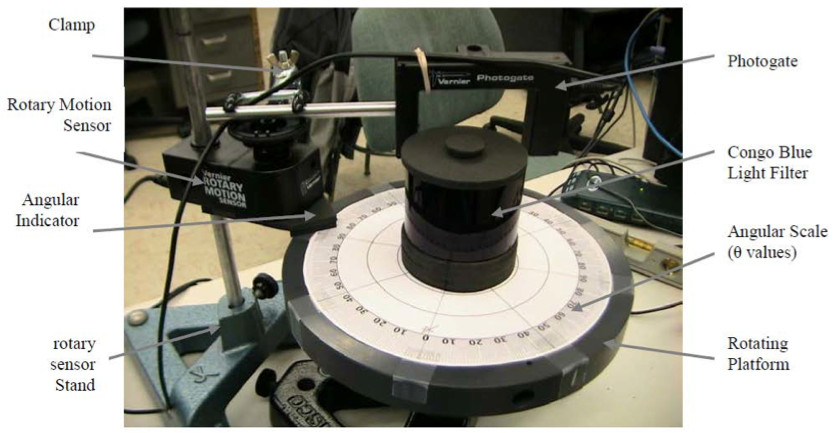
\includegraphics[width=0.6\textwidth]{opticalct.png}
\end{center}

There is more helpful information at http://web.pdx.edu/\~{}ralfw/ct.html


\newpage

%\section*{Project 8: Guided Surgery Tracking}
%
%Image-guided surgery technology has revolutionized traditional surgical techniques by providing surgeons
%with a way to navigate through the body using three-dimensional (3D) images as their guide. 
%Furthermore, those
%images can be changed, manipulated and merged to provide a level of detail not seen before in the operating room.
%The technology is similar to that used by todayÕs global positioning satellite systems, which can track the exact
%location and direction of vehicles at any point on the globe. Because the view is so precise and so controllable, a
%surgeon can actually see where healthy tissue ends and a brain tumor begins, or precisely where on the spine to
%place a pedicle screw to maximize patient mobility.
%
%\par One way to track movement in real time and know where the scalpel is in relation to the patient and area of interest
%is to use an accelerometer. This measures acceleration in three axes due to both gravity and motion. If the start
%point is known, the integration of the output of a 3 axis accelerometer can used to determine current location.
%Accelerometer chips are found in everything from Wii remotes to iPhones. They work by measuring the
%displacement of a suspended mass using changes in capacitance, but fortunately output the acceleration as an
%analog voltage. This voltage can be read and integrated in 3 dimensions in LabVIEW to give the current location.
%Attach an accelerometer to the end of a stylus and track its location. You could also do this with an Arduino.
%
%\begin{center}
%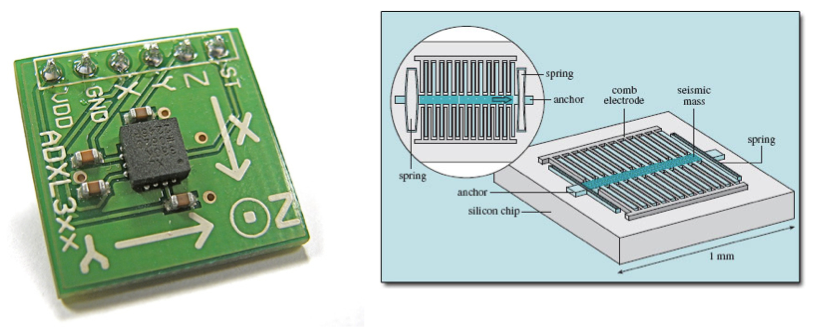
\includegraphics[width=\textwidth]{accelerometer.png}
%\end{center}
%
%\newpage

\section*{Project 8: Microsoft Kinect Gait Analysis}

Measuring gait is important in kinesiology and in monitoring people who have difficulty walking. 
There are lots of ways to measure gate, but the Microsoft Kinect gaming peripheral offers 
a particularly interesting and cheap way to do it. 
The Kinect has an IR projector and IR camera, and there is software available online to grab incoming image frames 
from the IR camera on a PC. 
The IR projector projects a grid of dots on a room that are used for depth analysis, 
which isn't particularly useful to us. 
Using IR has the advantage over visible light that it is easier to control its bright sources, 
which reduces noise and artifacts in images. 
There are at least two approaches that could be used to measure the position of a person's hips,
knees, and feet over time using the Kinect's IR camera:
\begin{enumerate}
\item Attach IR-reflective (retroreflector) tape bands to the waist, knees and feet and place an IR-diffusor over the projector, 
as described at:\\
 http://www.roborealm.com/tutorial/FIRST/slide010.php
\item Cover the IR projector with an opaque cover and attach battery-powered IR-LEDs to the joints. 
\end{enumerate}
Given captured IR image frames of a person walking past the camera, you will process them in MATLAB
to determine useful quantities such as step length and speed. 

%\section*{Project 9: 12-lead ECG}
%
%A clinical ECG measurement involves 10 electrodes to measure 12 different signals. 
%This gives information about different phases and directions of the heart depolarization in multiple dimensions.
%
%\par The following ECG leads are formed using instrumentation amplifier (INA128) and ECG electrode combinations:\\
%Lead I = LA Ð RA\\
%Lead II = LL Ð RA\\
%Lead V1 = V1 - (LA + RA + LL) / 3\\
%Lead V2 = V2 - (LA + RA + LL) / 3\\
%Lead V3 = V3 - (LA + RA + LL) / 3\\
%Lead V4 = V4 - (LA + RA + LL) / 3\\
%Lead V5 = V5 - (LA + RA + LL) / 3 Lead V6 = V6 - (LA + RA + LL) / 3\\
%
%\par Eight ECG lead data from the MBF filter is fed to the ECG lead formation module.
% This module computes the remaining four ECG lead data using the following formula:\\
%Lead III = Lead II - Lead I\\
%Lead aVR = - Lead II + 0.5 * Lead III\\
%Lead aVL = Lead I - 0.5 * Lead II Lead aVF = Lead III + 0.5 * Lead I\\
%
%See http://www.ti.com/lit/an/sprab36b/sprab36b.pdf for more information.
%
%\begin{center}
%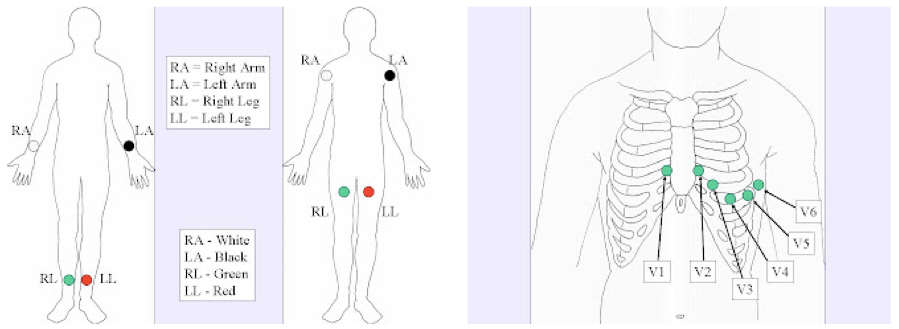
\includegraphics[width=\textwidth]{12leadecg.png}
%\end{center}

\newpage

\section*{Project 9: Automatic blood pressure measurement}

Blood pressure is most commonly measured by determining the onset of turbulent blood flow in the arteries using a pressure cuff and a sphygmanometer. 
Build an automatic blood pressure monitor that pumps up the cuff then listens for the onset of turbulent flow in LabView to determine systolic and diastolic pressure.

\newpage

\section*{Project 10: Spirometer}

Build a spirometer to characterize lung function by measuring volumetric airflow.
A spirometer is a device that measures breath, as characterized by the volume and speed of inhaled and exhaled air.
It is an important tool in assessing lung function, and diagnosing diseases such as asthma and pulmonary fibrosis.
Below-average spirometry values indicate that a patient's lungs are not functioning well.

\par The most basic maneuver of a spirometry test is to forcibly exhale a full inspiration and measure
the volume of exhaled air.
This is called Forced Vital Capacity (FVC), and you will measure it, 
along with Forced Expiratory Volume (FEV) in the first second
of exhalation (FEV$_1$). 
The ratio FEV$_1$/FVC is around 75-80\% in healthy adults.
In addition to this, you will measure Peak Expiratory Flow (PEF), 
which is the maximum flow rate achieved by forced exhalation after full inhalation.


\subsubsection*{Your Spirometer}
The device you will build will be based on transducing the pressure difference $\Delta p$ in a Venturi tube to a voltage signal that you will
condition, digitize, and process in LabView.
\begin{figure}[!h]
\begin{center}
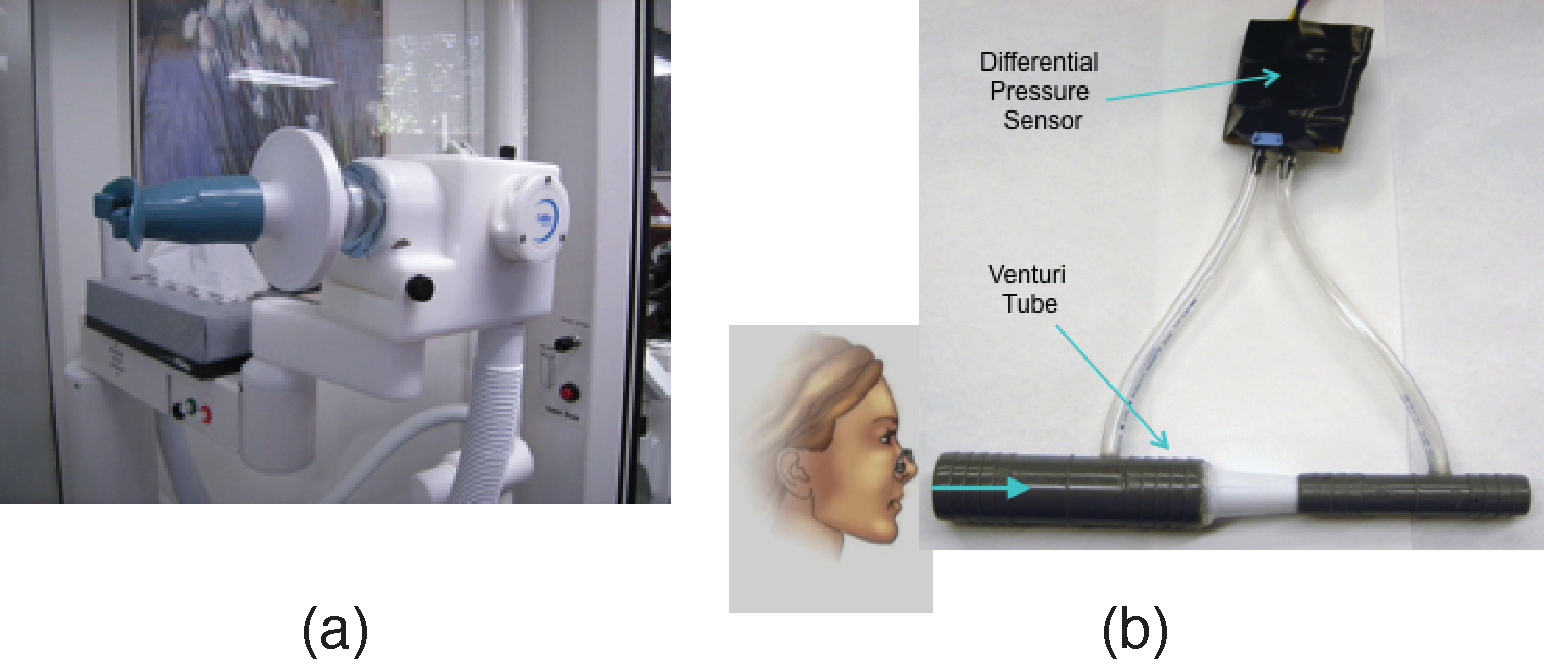
\includegraphics[width=\textwidth,trim=0 0 0 0,clip=false]{spirometerillustration.pdf}
\caption{(a) A clinical spirometer. (b) Illustration of the spirometer you will build, 
which is based on measuring the pressure difference between two sections of a Venturi tube
with different diameters.}
\label{fig:spirometer}
\end{center}
\end{figure}

%\begin{figure}[!h]
%\begin{center}
%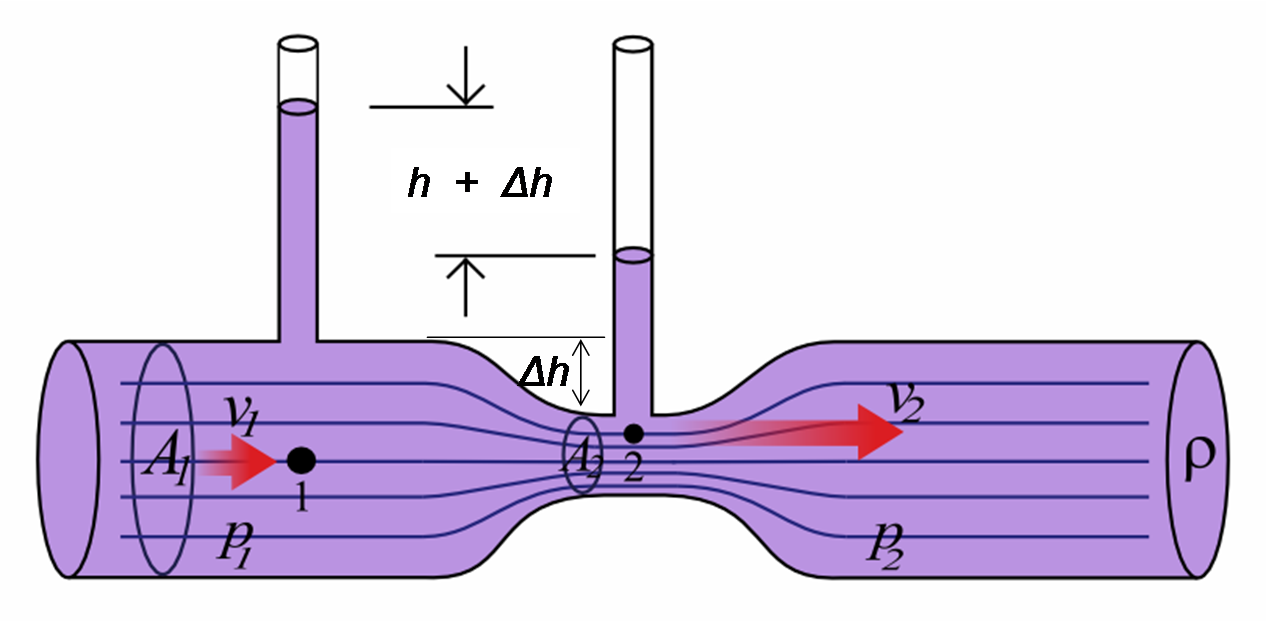
\includegraphics[width=0.75\textwidth,trim=0 0 0 0,clip=false]{Venturifixed2.PNG}
%\caption{Venturi tube.}
%\label{fig:venturi}
%\end{center}
%\end{figure}

\noindent The technical objectives of this project are to:
\begin{enumerate}
\item Measure the pressure difference in a Venturi tube using electronic sensors.
\item Condition the signal.
\item Read the signal using your NI DAQ card, convert the signal to quantitative units and analyze the data with LabView.
\item Make it work on an Arduino and make it battery-powered with a display!
\end{enumerate}

\newpage

\section*{Project 11: Arduino Theremin}

A theremin is a musical instrument comprising an oscillator attached to a speaker,
whose amplitude and frequency the musician can modulate by moving their hands 
closer or farther from antennas. 
This modulates the capacitance of the antennas, and the instrument transduces
those capacitances into control signals. 
This can be done with relatively simple circuits and the Arduino, for example here:\\

http://playground.arduino.cc//Main/CapacitiveSensor?from=Main.CapSense\\

and here:\\

http://medialappi.net/lab/tutorials/capacitive-sensing-with-arduino/\\

Another approach would be to use a function generator and a capacitance-to-voltage conversion circuit as discussed in class.
Build an Arduino or LabView theremin with two antennas using one of the approaches.
You should aim to provide the musician with a decent range of hand motion (i.e. more than just an inch or two). 
Use the measured voltages to control the pitch and volume of a computer-synthesized tone (for example by sending serial commands from the Arduino to the free Pure Data software). 
Can you quantitatively measure the capacitance? 

\newpage

\section*{Project 12: Video-based heart rate monitor}

Implement a simplified version of the method described in the paper at:
\begin{center}
 http://dl.acm.org/citation.cfm?id=2185561 
 \end{center}
 in MATLAB, LabView, or the like, and use it to detect heart rate when focusing a web cam or other camera at a subject's wrist or face. 

\begin{center}
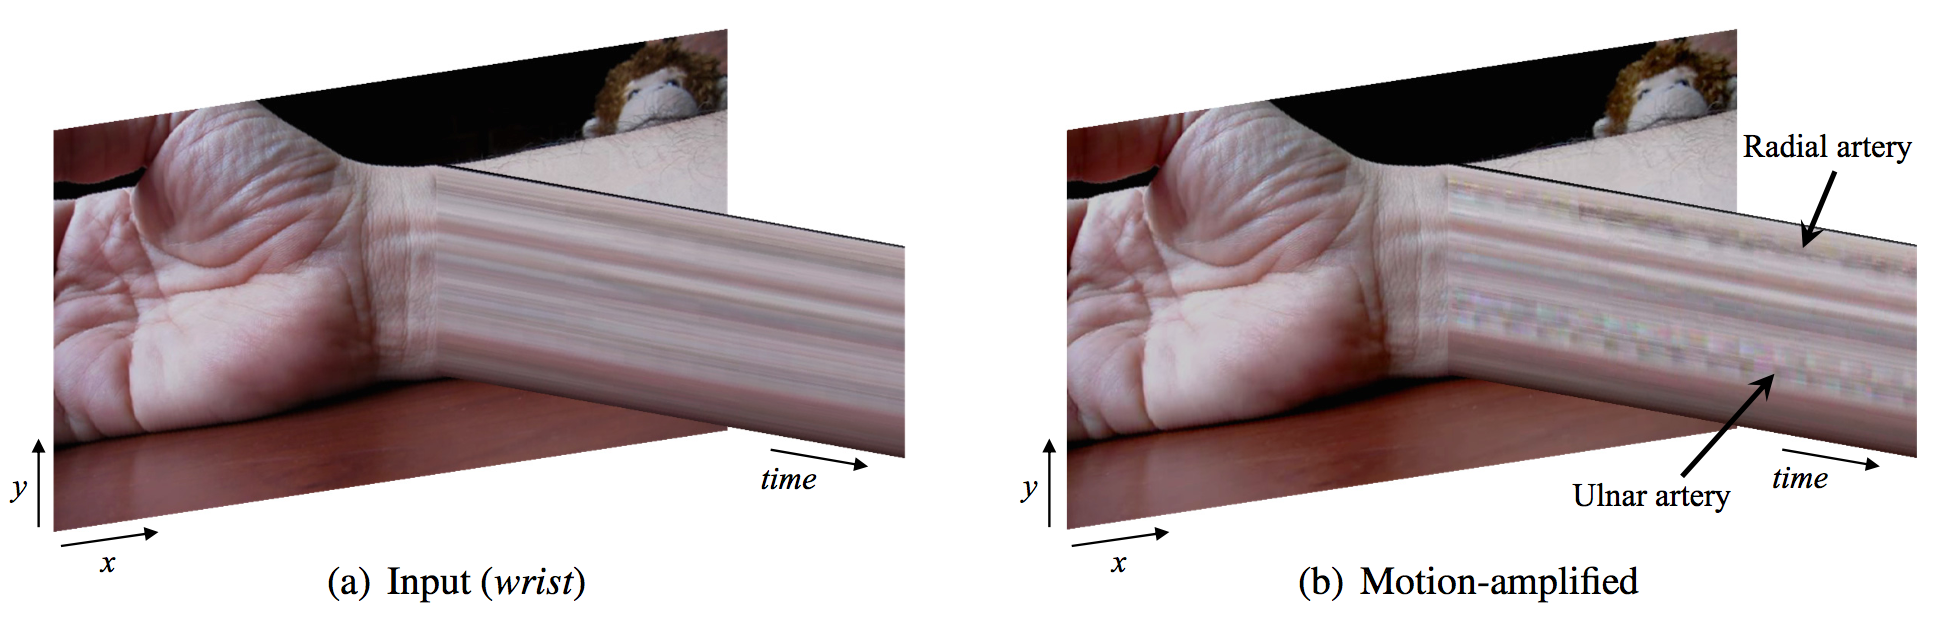
\includegraphics[width=\textwidth,trim=0 0 0 0,clip=false]{wrist_heartrate.png}
(Figure taken from referenced paper)
\end{center}

\newpage 
\section*{Project 13: Metal detector for MRI screening}

Implanted metal can be torqued by the main magnetic field of an MRI scanner,
ripping tissue, 
and RF burns can be caused by electric currents induced on the metal. 
For these reasons it is critical to screen patients for embedded metal before they enter the 
scanner. 
Build a metal detector that is capable of detecting surgical clips and other implanted metal.
The detector should be able to detect metal deposited deep inside a patient's torso.
Interestingly, it is possible to build a metal detector from just an AM radio and a calculator! 
But this will likely not be very sensitive. 

%
%
%\newpage
%
%\section*{Project 14: Radar velocity measurement}
%


%\subsection*{Steps}
%\begin{enumerate}
%
%\item Build the circuit in Fig. \ref{fig:circuit} on a breadboard. 
%When connecting the differential pressure sensor, check the pinout diagram of the pressure sensor on the attached datasheet.
%\begin{figure}[!h]
%\begin{center}
%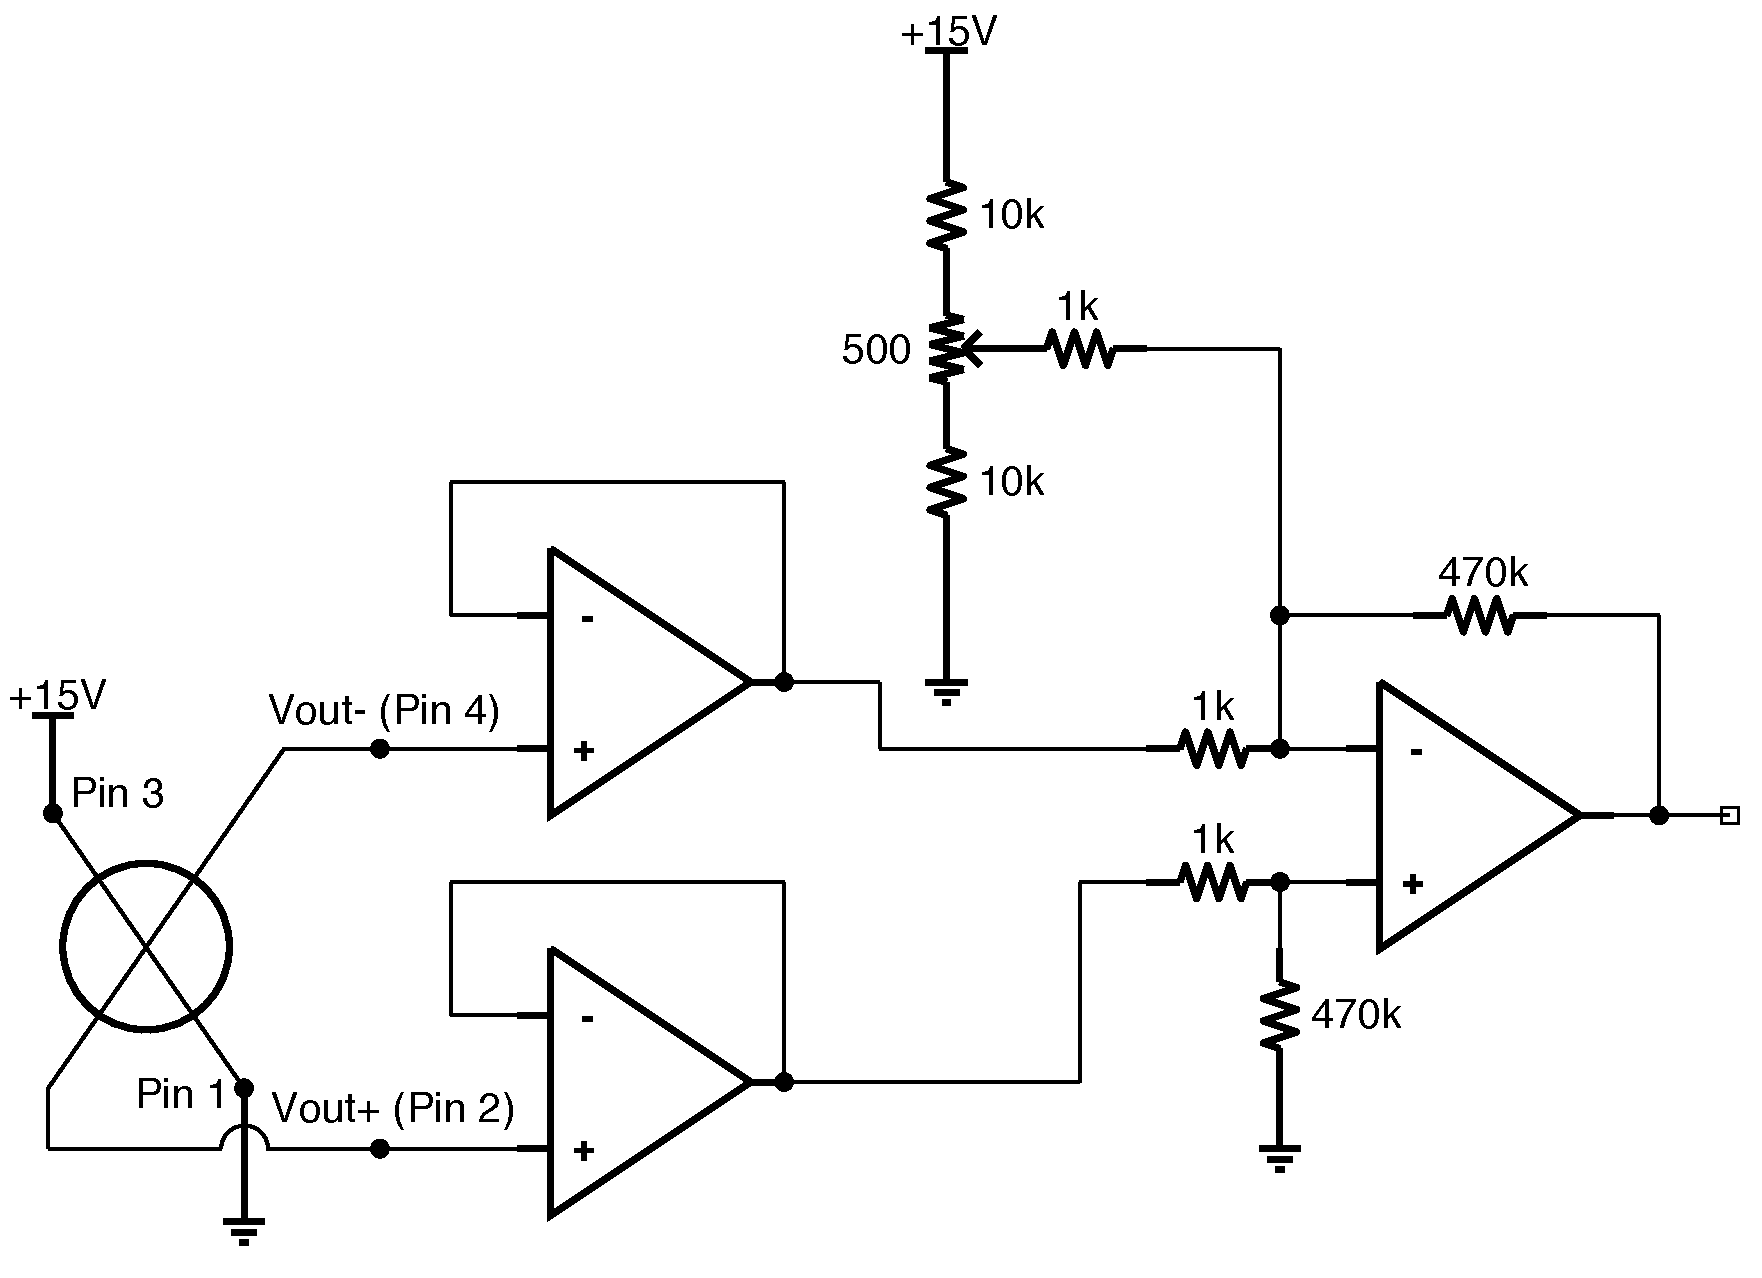
\includegraphics[width=\textwidth,trim=0 0 0 0,clip=false]{lab5circuit.pdf}
%\caption{Pressure sensor and amplifier circuit to build.}
%\label{fig:circuit}
%\end{center}
%\end{figure}
%
%\item Connect the output of the circuit to your DAQ board, with the ground switch set to (FS). 
%In the DAQ Assistant Express VI, select Continuous sampling, 100 Samples, 1 kHz rate, 
%and max/min input voltages of $\pm$10 V.
%Make a waveform chart in LabView. 
%Why is the noise so much lower in these than in the ECG?
%
%\item The tunable DC offset (at the top of the circuit schematic) can be used to cancel out a small DC differential voltage that you will observe at the output of the transducer. 
%Watching the measured signal in Labview, tune the DC offset to get zero output, with the pressure sensor plugged in.
%Note that the required offset may change a bit as as the transducer warms up, so you may want to check the offset again a few minutes after powering up the sensor.
%To remove this offset more robustly, you can place another DAQ Assistant outside of the first loop, set to 1 iteration, and set the DAQ to collect about 100 samples. 
%Then you can average that output and subtract it from the signal coming out of your main DAQ assistant. 
%This way, the average offset will be measured and subtracted each time your VI starts.
%
%\item Connect the Venturi tube to your sensor. 
%Note that the sensor expects the higher pressure from the wider pipe to come into Port \#1, 
%and the lower pressure from the narrower pipe to come into Port \#2.
%
%\item Filter your digitized signal in LabView. 
%In setting the filter parameters, keep in mind that your signal of interest has frequencies components mostly between 0 and 5 Hz.
%
%\item Convert your measured (and filtered) voltage to pressure (Pa or kPa), using the fact that the gain on your amplifier is 470, and (as is listed on the datasheet) 0.8 mV/kPa is your sensitivity. You can implement the conversion using the Formula Express VI. Make a chart for the pressure.
%
%\item Convert the measured pressure to flow rate (L/s), using Eq. \ref{eq:venturi} and the fact that the tubing diameters are 14.5 mm and 5.5 mm. You can implement the conversion using the Formula Express VI. Note that to convert from (m$^3$/s) to (L/s) you must multiply by 1000. Make a chart for the flow rate.
% 
%\item Use the Time Domain Math Express VI (select `Calculate Integral') to integrate your flow rate over time, yielding a Volume signal. 
%Make a chart for this signal.
%The value of this signal at the end of a forced exhalation is the FVC. 
%Measure and record FVC, FEV$_1$, and FEV$_1$/FVC for each member in your group. 
%We recommend using alcohol swabs to sanitize the mouthpiece between users.
%
%\item Create a Flow vs Volume Graph - the X-axis will be Volume, and the Y-Axis will be Flow. This will be an X-Y graph, rather than a standard chart. 
%Then attach the flow rate and the Volume to this. The result you see during a forced exhale should look like the top part of the graph in Fig. \ref{fig:fvsv}.
%What does this chart tell you about the relationship between Flow and Volume during a forced exhalation?
%
%%\begin{figure}[h]
%%\begin{center}
%%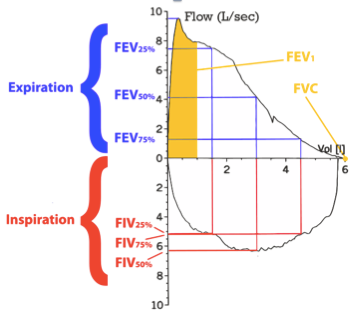
\includegraphics[width=0.5\textwidth,trim=0 0 0 0,clip=false]{flowvsvolume.png}
%%\caption{A typical flow vs volume curve for expiration and inhalation.}
%%\label{fig:fvsv}
%%\end{center}
%%\end{figure}
%
%\item At some point, validate your volume measurements using the 3 L syringe. 
%What are the potential sources of error in your measurements?
%
%\item Since the sensor can only measure unidirectional flow, how could you go about measuring Tidal Volume? 
%Implement your idea.



%\end{enumerate}

\end{document} 